\section{Extended example}
\label{sec:imperative-balltracker}
To get a better feel for how a feedback control system works in practice, we will discuss a simple but interesting application of feedback control that uses the theory covered in the previous sections. In this section we show an imperative reference implementation. In the next chapter we will continue to use and refactor this application as we come up with an API for constructing and executing feedback systems. The application at hand is a port from the original implementation by Nikita Leshenko in Javascript, CSS and HTML \cite{nikital-balltracker}. We will however use Scala as our programming language and JavaFx for drawing the graphics on the screen. To get a feel of what this application is doing we strongly recommend to have a look at the online version\footnote{\url{http://nikital.github.io/pid/}} first before proceeding with this section!

The application consists of a flat surface on which a ball can move around. The goal is to move the ball from its initial position to the position on the surface that the user clicks on with the mouse. \Cref{fig:balltracker-initial} shows the ball in its initial state when the application starts. When the user clicks on the screen, the ball starts moving to that position as shown by \Cref{fig:balltracker-moving}. Besides the background and the ball, also the desired position, a dashed line between the ball and the desired position, the acceleration in both the $x$ and $y$ directions and a trail of previous positions are drawn (which are fading away over time). After some time the ball is at its desired position and waits there for a new position to navigate to, as is shown in \Cref{fig:balltracker-reached}. Notice that the desired position can also be updated while the ball is still moving, in which case it moves to the new and discards the old destination.

\begin{figure}
	\centering
	\begin{subfigure}[b]{0.80\linewidth}
		
\includegraphics[trim = 0mm 110mm 0mm 0mm, clip, width=\linewidth]{figures/BallTracker-initial.png}
		\caption{Initial}
		\label{fig:balltracker-initial}
	\end{subfigure}
	
	\begin{subfigure}[b]{0.80\linewidth}
		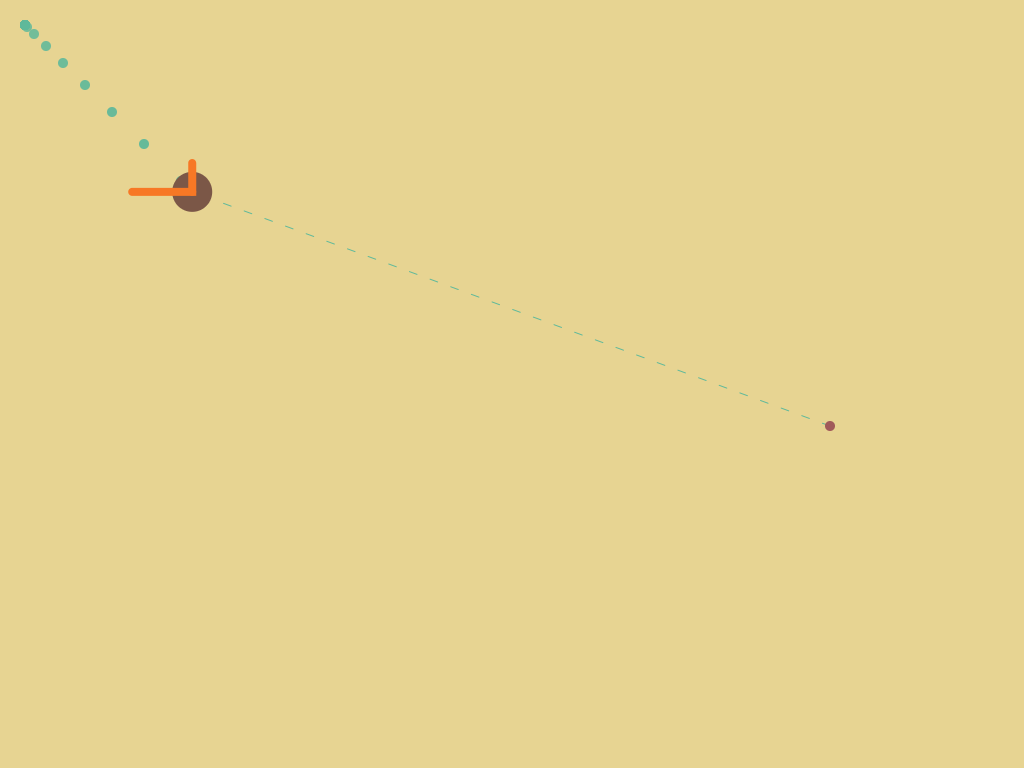
\includegraphics[trim = 0mm 110mm 0mm 0mm, clip, width=\linewidth]{figures/BallTracker-moving.png}
		\caption{Moving to desired position}
		\label{fig:balltracker-moving}
	\end{subfigure}
	
	\begin{subfigure}[b]{0.80\linewidth}
		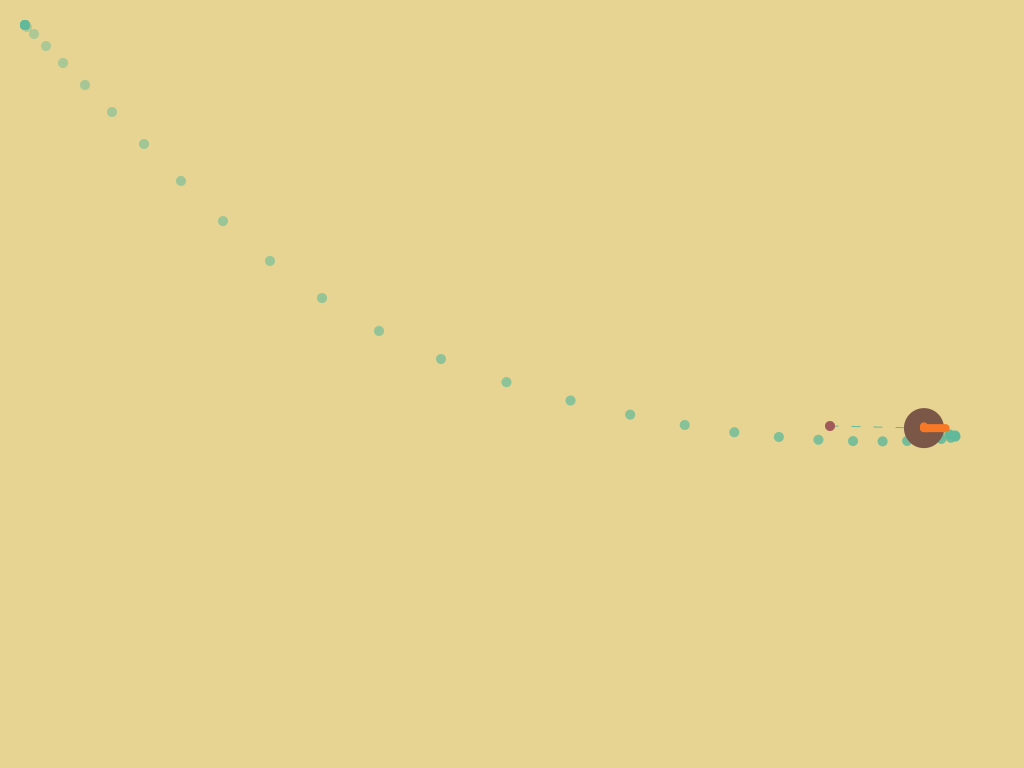
\includegraphics[trim = 0mm 110mm 0mm 0mm, clip, width=\linewidth]{figures/BallTracker-overshooting.png}
		\caption{Moving to desired position, overshooting a bit}
		\label{fig:balltracker-moving}
	\end{subfigure}
	
	\begin{subfigure}[b]{0.80\linewidth}
		
\includegraphics[trim = 0mm 110mm 0mm 0mm, clip, width=\linewidth]{figures/BallTracker-desired.png}
		\caption{Reached desired position}
		\label{fig:balltracker-reached}
	\end{subfigure}
	\caption{Ball movement}
	\label{fig:balltracker}
\end{figure}

In order to allow the ball to move in a natural way, we remind the reader of some basic equations from physics that describe the one dimensional motion of an object as a function of time (\Cref{eq:motion}). Here $x_t$, $v_t$ and $a_t$ are the ball's position, velocity and acceleration at time $t$ respectively. For two-dimensional motion we can combine two sets of these equations for both dimensions.

\begin{subequations}
	\begin{equation}
		x_t = x_{t - 1} + v_t \cdot \Delta t
	\end{equation}
	\begin{equation}
		v_t = v_{t - 1} + a_t \cdot \Delta t
	\end{equation}
	\label{eq:motion}
\end{subequations}

The implementation of these required pieces of physics can be found in \Cref{lst:ball-physics}. We first define a \code{Position}, \code{Velocity} and \code{Acceleration} as tuples of \code{Double} as well as some mathematical operations on the tuple type. The \code{Ball} class describes the state of the ball having a position, velocity and acceleration. A second constructor (\code{apply}) defines the initial position with no acceleration or velocity. The method \code{accelerate} on this class takes a new acceleration and calculates a new state for the ball according to \Cref{eq:motion}. Notice that we discard the $\Delta t$ term, since this will always be equal to 1. To keep track of the ball's previous positions we define \code{History} to be a queue of \code{Position}s.

\begin{minipage}{\linewidth}
\begin{lstlisting}[style=ScalaStyle, caption={Ball motion physics}, label={lst:ball-physics}]
type Position $=$ (Double, Double)
type Velocity $=$ (Double, Double)
type Acceleration $=$ (Double, Double)
type History $=$ mutable.Queue[Position]

implicit class Tuple2Math[X: Numeric, Y: Numeric](val src: (X, Y)) {
  import Numeric.Implicits._
  def +(other: (X, Y)) $=$ (src._1 + other._1, src._2 + other._2)
  def -(other: (X, Y)) $=$ (src._1 - other._1, src._2 - other._2)
  def *(scalar: X)(implicit ev: Y $=:=$ X) $=$ (scalar * src._1, scalar * src._2)
  def map[Z](f: X $\Rightarrow$ Z)(implicit ev: Y $=:=$ X): (Z, Z) $=$ (f(src._1), f(src._2))
}

case class Ball(acc: Acceleration, vel: Velocity, pos: Position) {
  def accelerate(newAcc: Acceleration) $=$ Ball(newAcc, vel + newAcc, pos + vel + newAcc) |\label{line:accelerate}|
}
object Ball {
  def apply(radius: Double) $=$ Ball((0.0, 0.0), (0.0, 0.0), (radius, radius))
}
\end{lstlisting}
\end{minipage}

The next step in creating this application is to design the feedback system itself (\Cref{fig:balltracker-diagram}). The \textit{system under control} here is of course the ball, from which at any point acceleration, velocity and position can be measured. Given that our \textit{setpoint} is equivalent to the position of where the ball should end up eventually, it makes most sense to define the \textit{control output} as the current position of the ball. From this it follows that the \textit{tracking error} represents the distance to be traveled before reaching the desired position. Depending on the distance, a controller can then decide how much it wants to speed up the ball by providing a new acceleration as the system's \textit{control input}. To get the ball's next position, this acceleration has to be integrated twice to get the ball's position after $\Delta t$ time.

To transform a distance into an acceleration, we can use the power of the PID controller. As discussed before this controller is renowned for its effectiveness and simplicity and is therefore most commonly used in all kinds of feedback systems, especially those who deal with floating point control inputs and outputs. For this use case it makes absolute sense to use this controller as well. The \textit{proportional controller} will look at the current distance to be traveled and comes up with some amount of acceleration. However, this acceleration will approach zero as the ball approaches its destination, causing it to keep its same velocity rather than slowing down. To prevent this, we need a strong \textit{derivative controller} that can counteract this velocity and slow down the ball as the distance is becoming smaller. For the purpose of looking back at previous distances we also add an \textit{integral controller} into the mix.

\begin{figure}[H]
	\begin{center}
		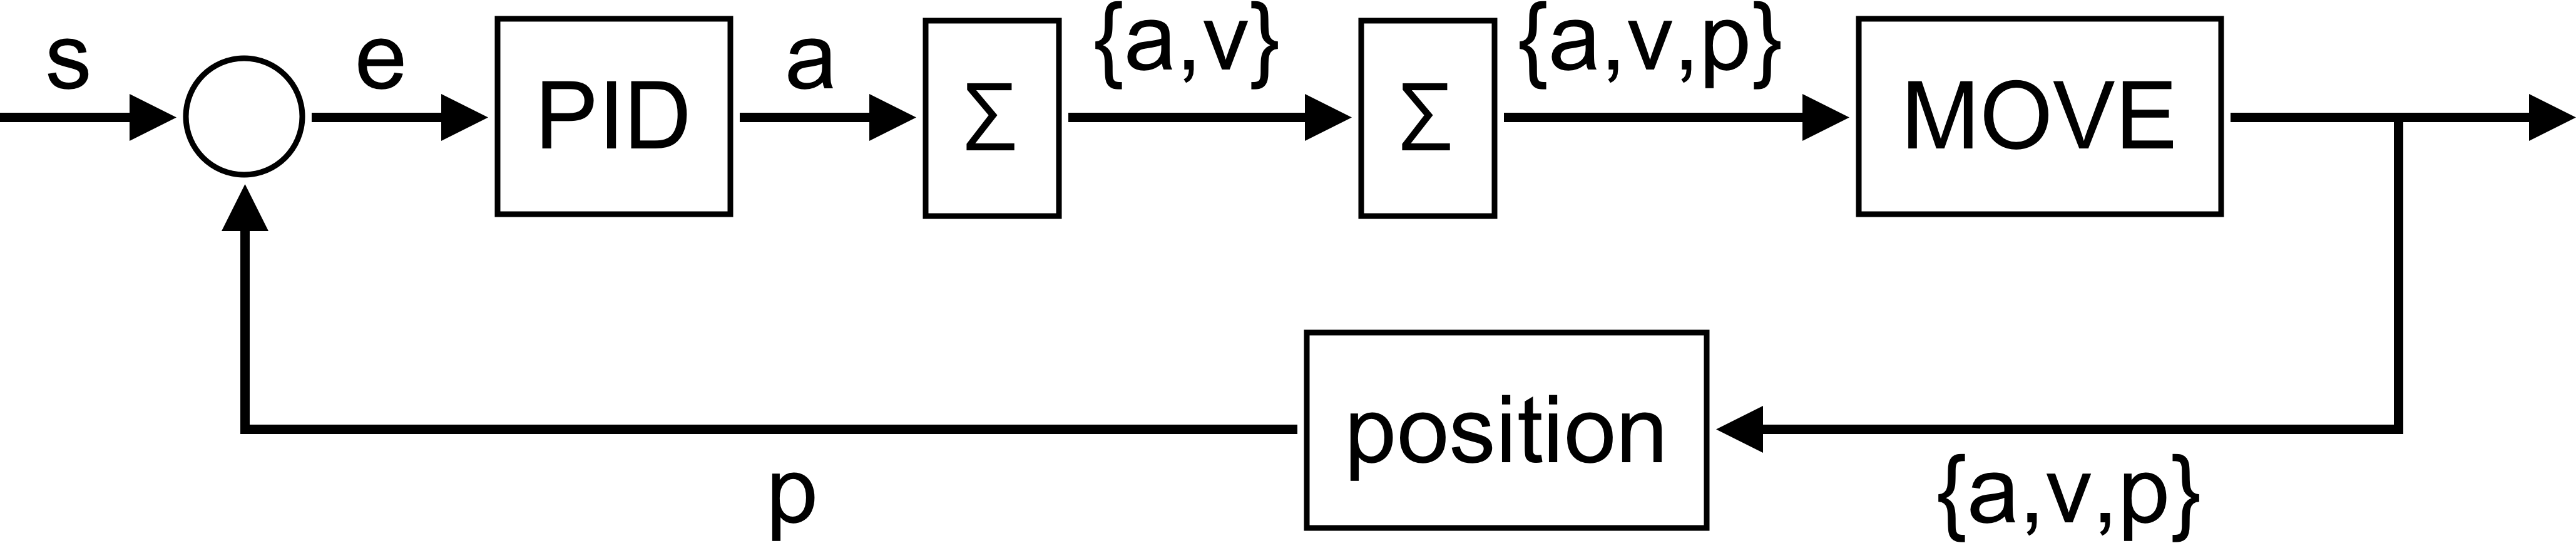
\includegraphics[width=0.85\textwidth]{figures/BallTracker-diagram.png}
	\end{center}
	\caption{Architecture of the ball movement control system}
	\label{fig:balltracker-diagram}
\end{figure}

Both the PID controller and the feedback system are implemented in \Cref{lst:ball-feedback}. After some initialization we define an iteration of the controller following \Cref{eq:proportional-control,eq:integral-control-discrete,eq:derivative-control} in the \code{pid} function on \cref{line:pid-function}. Again notice that this operates on the tuple types and uses the operators defined in \Cref{lst:ball-physics}. This function returns a new \code{Acceleration} which corresponds to the control input as described above.

The PID controller is then used in the construction of the feedback cycle (\cref{line:update}). It is first scaled down in such a way that it has an absolute maximum acceleration $0.2$, after which it is fed into the controlled system. This calls the \code{accelerate} function on the \code{Ball} (\Cref{lst:ball-physics} \cref{line:accelerate}), which calculates the ball's new velocity and position. The new state is then stored in the \code{ball} variable, which represents the latest control output. The rest of this function deals with managing the history and redrawing the application, which are considered not relevant for the implementation of the feedback system itself. The omitted code can be found in \Cref{app:ball-movement}.

Now that the feedback cycle is implemented, we can plug this in a JavaFx application that contains the canvas on which the application is drawn, as well as assigning the setpoint value and looping through the feedback cycle every 16 milliseconds. The code for this can be found in \Cref{app:ball-movement} as well.

Notice that with this feedback system we lack the notion of an external disturbance on the system under control. In this case there is none since the system is just the two \textit{sigma}s and the \textit{DRAW}. One could argue that the changing setpoint is kind of a disturbance, although this is by definition not the case. An example of an external disturbance on this particular system could be the terrain not being flat but rather containing hills and valleys. This would influence the ball's movement because of gravity, which would add a force in a third direction. For the sake of simplicity of this example we decided to not add this feature and stick with the flat terrain. We leave implementing this feature as an exercise to the reader.

\begin{minipage}{\linewidth}
\begin{lstlisting}[style=ScalaStyle, caption={Ball drawing}, label={lst:ball-feedback}]
var ball $=$ Ball(ballRadius)
var setpoint $=$ ball.position
var prevError, integral $=$ (0.0, 0.0)

// initializing history
// ...

def pid: Acceleration $=$ { |\label{line:pid-function}|
  val (kp, ki, kd) $=$ (3.0, 0.0001, 80.0)
  val error $=$ setpoint - ball.position
  val derivative $=$ error - prevError

  integral $=$ integral + error
  prevError $=$ error

  (error * kp + integral * ki + derivative * kd) * 0.001
}

def update(implicit gc: GraphicsContext): Unit $=$ { |\label{line:update}|
  val acceleration $=$ pid.map(a $\Rightarrow$ math.max(math.min(a, 0.2), -0.2))
  ball $=$ ball.accelerate(acceleration)

  // managing the history
  // ...

  // drawing all the elements
  // ...
}
\end{lstlisting}
\end{minipage}

\subsection*{PID control tuning}
As one can see from the code, there is not much room in the feedback system to work on the performance or accuracy of the ball movement control. The controlled system, in \Cref{fig:balltracker-diagram} consisting of the two \textit{sigma}s and the \textit{DRAW}, is fixed by the equations in \ref{eq:motion}. Also the \textit{position} block is not something that can improve the performance and accuracy. The only place to do so are the three controller gains in the PID controller function. In \Cref{lst:ball-feedback} \cref{line:pid-function} we set these values to $k_p = 3.0$, $k_i = 0.0001$ and $k_d = 80.0$\footnote{We will refer to these values as \textit{default values}.}. These values originate from the original version of this application by Nikita Leshenko \cite{nikital-balltracker}. In his implementation one can also alter these values and see how they affect the performance and accuracy of the ball movement.

In this section we will discuss some effects of the controller gains by altering the default values and observing how they alter the behavior of the ball's movement. For this we scale down the original application to 1 dimension, initialize the ball at position 20 (the ball is 20 units wide on the screen) and set the ball's setpoint at position 500. We let the ball move from its original position to the setpoint and meanwhile record the proportional, integral and derivative controller that make up the PID controller as well as the total acceleration\footnote{This is the acceleration before multiplying it with $0.001$ and maximizing it at $0.2$} and the balls position after applying the newest acceleration. We then plot these results, where the horizontal axis represents time, the primary vertical axis represents the accelerations and the secondary vertical axis represents the ball's position. The default behavior of the application is shown in \Cref{fig:balltracker-pid-default}.

We already discussed the setting of only having a proportional gain (set $k_i$ and $k_d$ to zero): as the ball approaches its destination, its acceleration will approach zero, meaning that the ball will not slow down but will rather keep moving with the same velocity. The exact behavior can be seen in \Cref{fig:balltracker-pid-kp-only}.The acceleration becomes zero as the ball reaches its setpoint, but only slows down past this point. At the time the ball comes to a hold, the distance with the setpoint is thus large that it needs to accelerate again (in the other direction). This process will repeat itself indefinitely without ever coming to a halt at the setpoint.

\begin{figure}
	\centering
	\begin{subfigure}[b]{0.49\linewidth}
		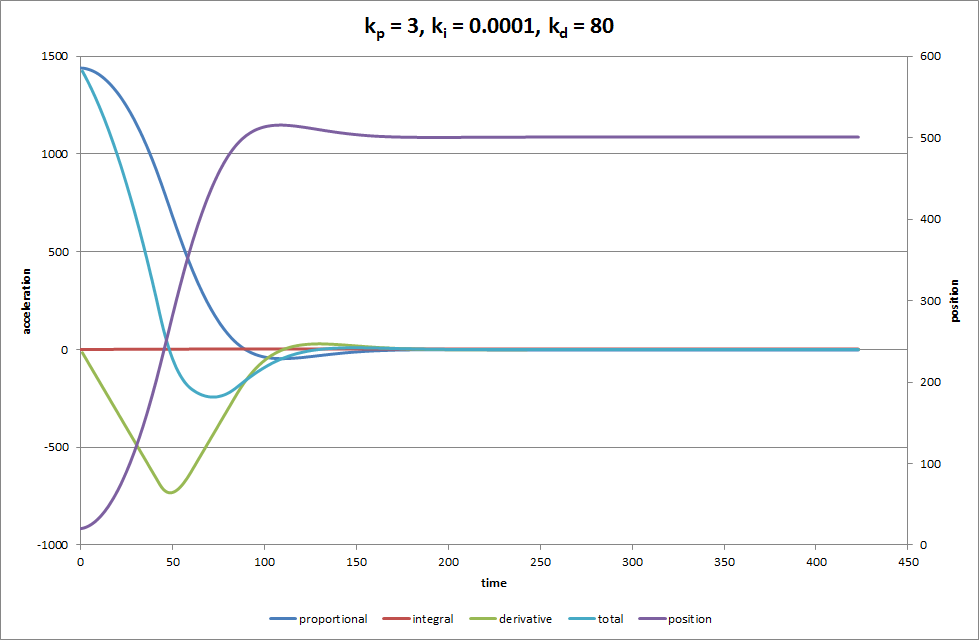
\includegraphics[width=\linewidth]{{figures/balltracker-pid/kp=3,ki=0.0001,kd=80}.png}
		\caption{$k_p = 3$, $k_i = 0.0001$, $k_d = 80$ (default)}
		\label{fig:balltracker-pid-default}
	\end{subfigure}
	\begin{subfigure}[b]{0.49\linewidth}
		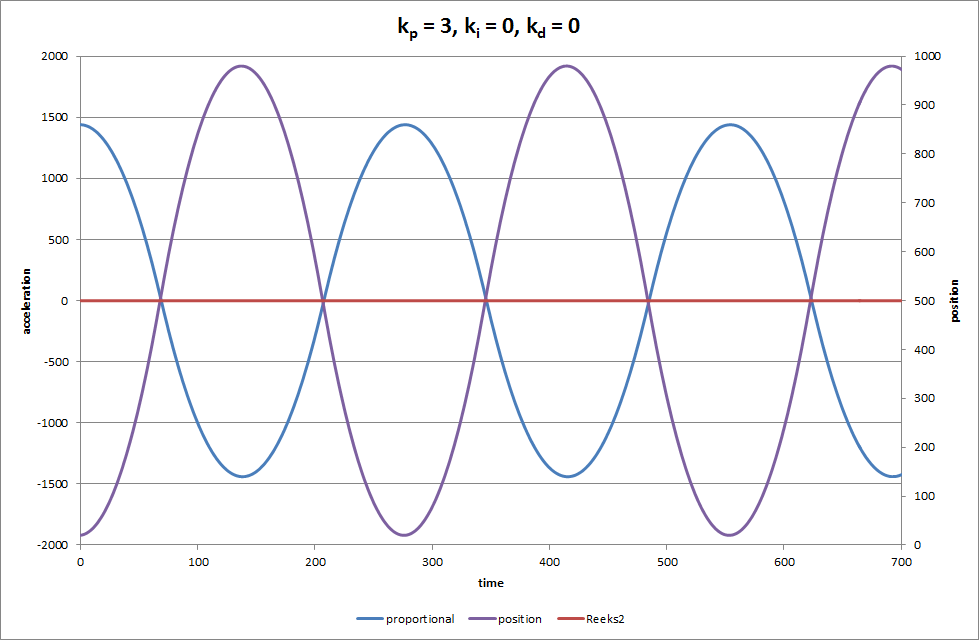
\includegraphics[width=\linewidth]{{figures/balltracker-pid/kp=3,ki=0,kd=0}.png}
		\caption{$k_p = 3$, $k_i = 0$, $k_d = 0$}
		\label{fig:balltracker-pid-kp-only}
	\end{subfigure}
	
	\begin{subfigure}[b]{0.49\linewidth}
		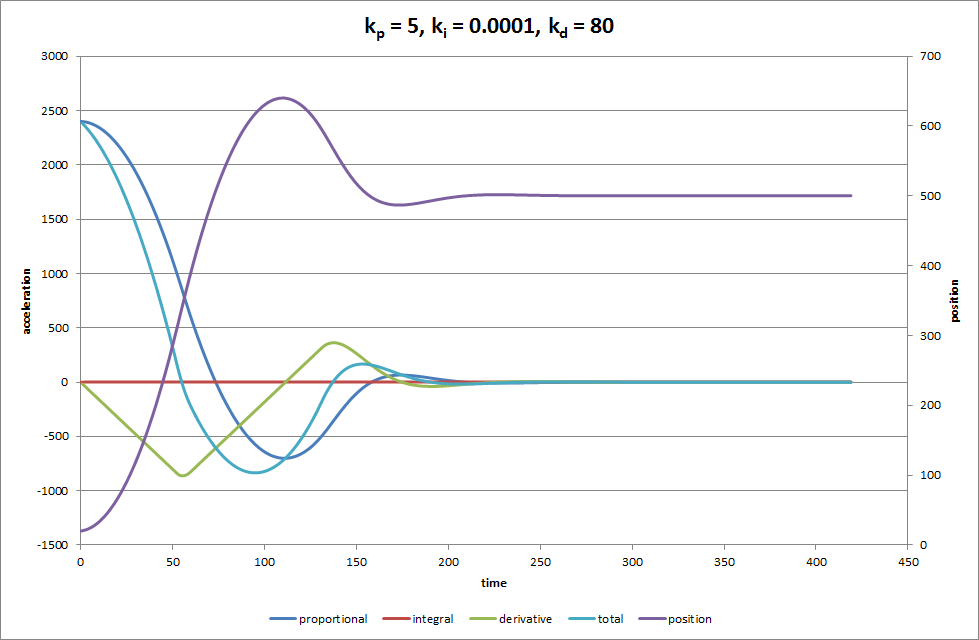
\includegraphics[width=\linewidth]{{figures/balltracker-pid/kp=5,ki=0.0001,kd=80}.png}
		\caption{$k_p = 5$, $k_i = 0.0001$, $k_d = 80$}
		\label{fig:balltracker-pid-kp-higher}
	\end{subfigure}
	\begin{subfigure}[b]{0.49\linewidth}
		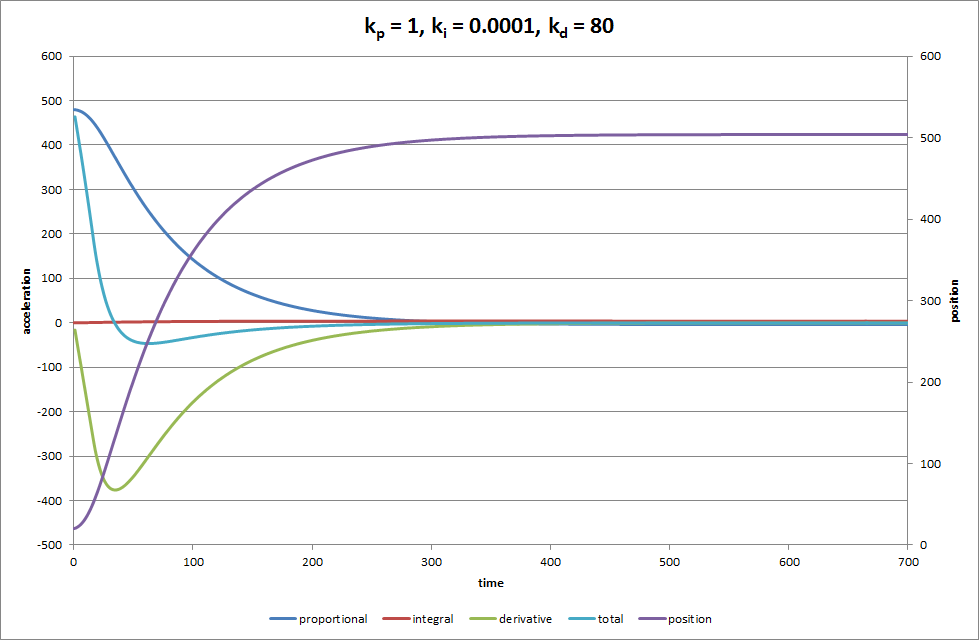
\includegraphics[width=\linewidth]{{figures/balltracker-pid/kp=1,ki=0.0001,kd=80}.png}
		\caption{$k_p = 1$, $k_i = 0.0001$, $k_d = 80$}
		\label{fig:balltracker-pid-kp-lower}
	\end{subfigure}
	
	\begin{subfigure}[b]{0.49\linewidth}
		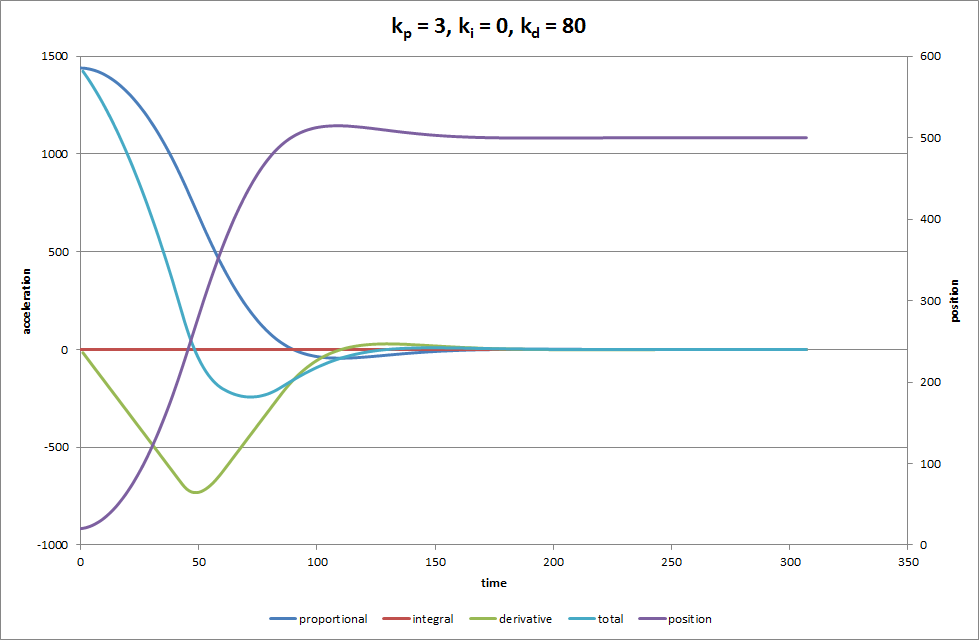
\includegraphics[width=\linewidth]{{figures/balltracker-pid/kp=3,ki=0,kd=80}.png}
		\caption{$k_p = 3$, $k_i = 0$, $k_d = 80$}
		\label{fig:balltracker-pid-ki-zero}
	\end{subfigure}
	\begin{subfigure}[b]{0.49\linewidth}
		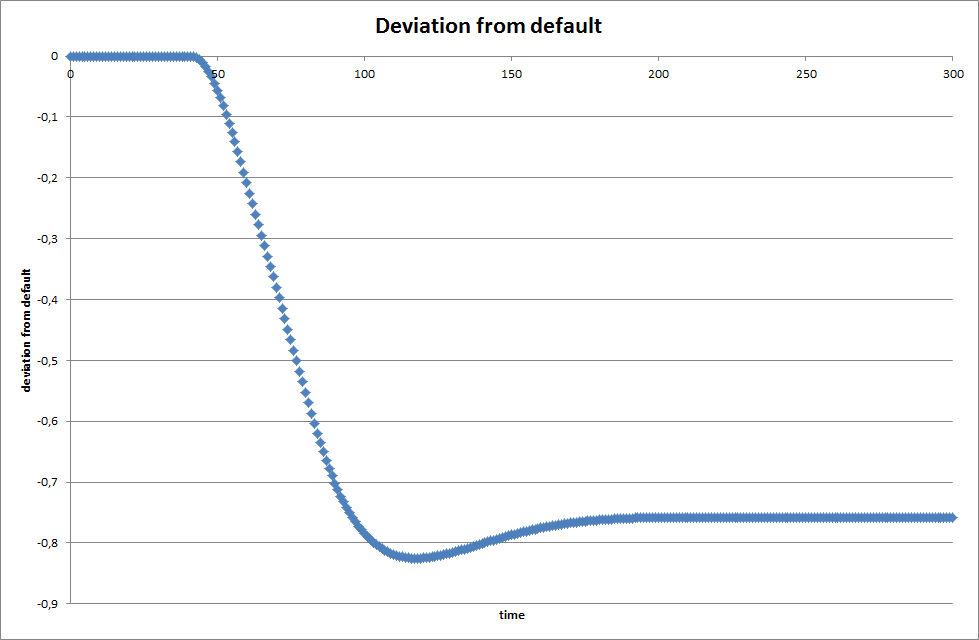
\includegraphics[width=\linewidth]{{figures/balltracker-pid/kp=3,ki=0,kd=80,diff}.png}
		\caption{$k_p = 3$, $k_i = 0$, $k_d = 80$}
		\label{fig:balltracker-pid-ki-zero-diff}
	\end{subfigure}
	
	\begin{subfigure}[b]{0.49\linewidth}
		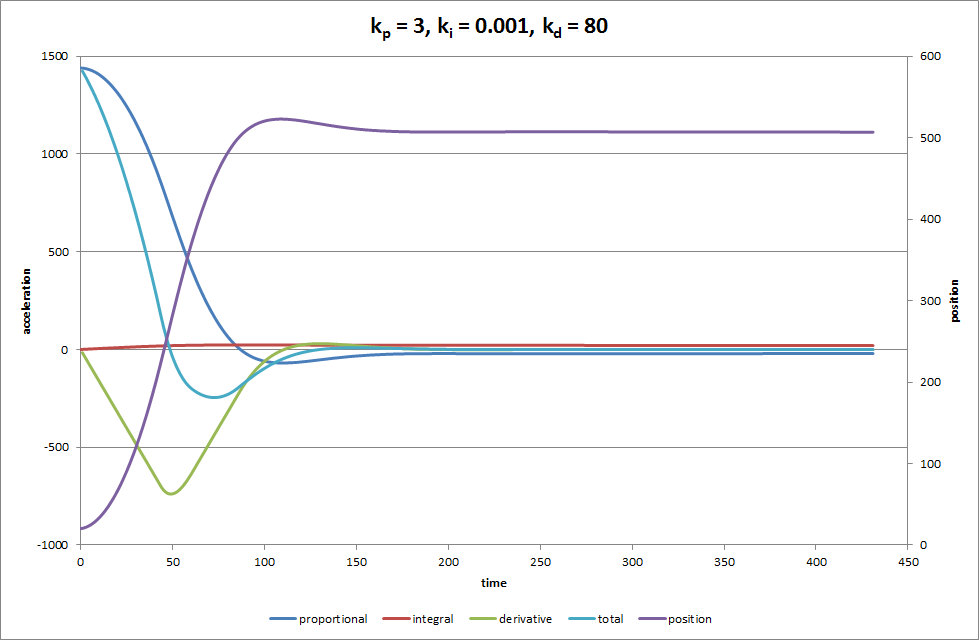
\includegraphics[width=\linewidth]{{figures/balltracker-pid/kp=3,ki=0.001,kd=80}.png}
		\caption{$k_p = 3$, $k_i = 0.001$, $k_d = 80$}
		\label{fig:balltracker-pid-ki-higher}
	\end{subfigure}
	\begin{subfigure}[b]{0.49\linewidth}
		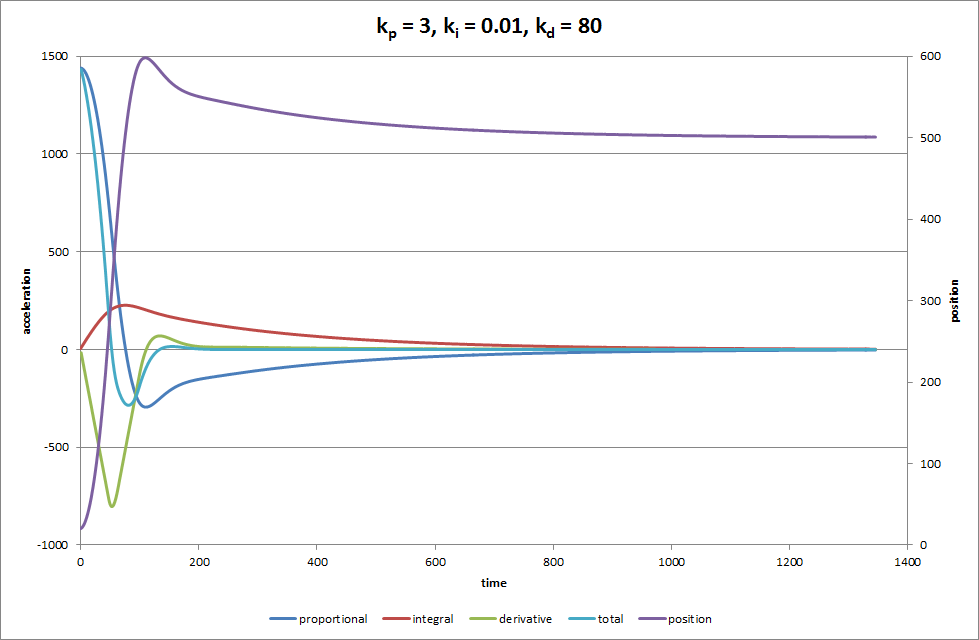
\includegraphics[width=\linewidth]{{figures/balltracker-pid/kp=3,ki=0.01,kd=80}.png}
		\caption{$k_p = 3$, $k_i = 0.01$, $k_d = 80$}
		\label{fig:balltracker-pid-ki-highest}
	\end{subfigure}
	\caption{Various values for the controller gains in a PID controller}
	\label{fig:pid-settings}
\end{figure}

On the other hand, altering the default settings with a larger value for proportional controller gain (for example $k_p = 5$) will cause the ball to overshoot its destination and have more oscillation around the destination before coming to a halt (\Cref{fig:balltracker-pid-kp-higher}). A smaller value ($k_p = 1$) will have the opposite effect (\Cref{fig:balltracker-pid-kp-lower}): it slows the ball down too early and also deviates a bit from the setpoint when it halts (position 503 where 500 was expected). This is expected and according to the theory as described earlier as well as by Janert \cite{janert2013-feedback}: a too high controller gain will cause overshooting the setpoint and oscillations, whereas a too low controller gain will cause undershooting and approaching the setpoint too slow.

The integral controller gain is set very low by default. This is no surprise, as the previous tracking errors (the distance still to be traveled) are not of much interest for the transformation to a new acceleration. As far as we were able to observe, discarding the integral factor complete does not really hurt the performance; in fact it only improves the accuracy (\Cref{fig:balltracker-pid-ki-zero,fig:balltracker-pid-ki-zero-diff}).

Increasing this value will however lead to some interesting behaviors. A value like $k_i = 0.001$ (10x higher than default) will cause the ball to end up slightly offset of its actual destination (\Cref{fig:balltracker-pid-ki-higher}). A value like $k_i = 0.01$ (100x the default value) has an even more peculiar behavior as it first approaches the destination in somewhat normal fashion, then almost stops at an offset position and creeps forward very slowly to the actual destination and holds at the correct position. This of course has to do with the relative weight of the integral part of the controller with regards to the weight of the proportional and derivative parts.

The derivative controller gain has the largest relative impact on the PID controller with its default value being set to $k_d = 80$. This value determines most of the oscillation in the system: the larger this value is, the less oscillation occurs. On the other hand, having a derivative controller gain that is too big is not good either as it will slow down the ball too early and make it creep towards its destination.

Tuning a PID controller is mainly a process of trial and error. One needs to find an optimal set of three values for the controller gains and with that has a very limited number of parameters to tune. For applications in physics there exist equations that give accurate values for these three parameters, although these only work correctly if the behavior of the system under control is fully known and can be translated in differential equations\footnote{Technically this could have been done for this example since it comes straight from physics, but for the sake of demonstrating it in the context of computer science we choose not to do so.}.

Janert spends a couple of chapters on the topic of controller tuning in de context of computer science \cite{janert2013-feedback} and goes into much detail to come up with equations that can give a first idea of the range in which to search for the optimal controller gains. This however are just an indication and still require experimentation to come up with the best solutions.
